\documentclass[letterpaper,11pt]{article}

\usepackage[margin=1in]{geometry}
\usepackage{times}
\usepackage{titlesec}
\usepackage{amsmath,amssymb,amsthm}
\usepackage{graphicx}
\usepackage[font=small]{caption}
\usepackage{subcaption}
\usepackage{hyperref}
\usepackage[T1]{fontenc}
\usepackage[giveninits=true]{biblatex}
%\usepackage[style=mla]{biblatex}
\usepackage{tabularx}
\usepackage{cleveref}
\usepackage{tikz}
\usepackage{wrapfig}

\usetikzlibrary{arrows.meta}
\usetikzlibrary{shapes.geometric}
\usetikzlibrary{shapes.multipart}
\usetikzlibrary{cd}

\addbibresource{publication24.bib}
\addbibresource{additional_ref.bib}

\graphicspath{
    {Figs/},{figures/}
}

\titlespacing{\paragraph}{0pt}{1ex}{0.4cm}

\newcommand{\cF}{{\mathcal{F}}}
\newcommand{\cX}{{\mathcal{X}}}

\newcommand{\dg}[1]{{\textcolor{blue}{#1}}}


\newwrite\loggraphics
\immediate\openout\loggraphics=\jobname.loggraphics%
\let\oincludegraphics\includegraphics% store original \includegraphics
\renewcommand{\includegraphics}[2][]{% prepend to it (could also use xpatch, etc.)
  \immediate\write\loggraphics{#2}
  \oincludegraphics[#1]{#2}}


\begin{document}

\thispagestyle{empty}
\noindent\textbf{ANNUAL REPORT}\\[1cm]
\centerline{\textbf{\Large Unified Large-Scale Theoretical and Computational Frameworks}}
\centerline{\textbf{\Large for Invariance and Composition of Open Hybrid Dynamical Systems}}\\[1cm]

\renewcommand\arraystretch{1.5}
\begin{tabularx}{1.0\textwidth}{>{\bfseries}lX}
Award Number & FA9550-23-1-0400\\
Report Type & Annual\\
Reporting Period & July 2, 2024 - July 1, 2025\\
Distribution Statement & Distribution A - Approved for public release\\
Program Officer Name & Dr. Frederick Leve\\
Principal Investigator Name & Dr. Taeyoung Lee\\
Project Title & Unified Large-Scale Theoretical and Computational Frameworks for Invariance and Composition of Open Hybrid Dynamical Systems\\
%
Abstract & 
This project aims to establish both theoretical and computational frameworks for analyzing and certifying the complex behaviors of open hybrid dynamical systems.
Our research is organized around three core themes.
First, we developed geometric and algebraic topological frameworks to uncover inherent structures in hybrid systems, such as topological features and invariants.
Second, we explored how these structures are influenced by uncertainty and by the composition of systems across complex networks.
Finally, we extended these insights to enable scalable control, optimization, and learning for high-dimensional hybrid systems.
Collectively, these efforts provide a rigorous, unifying foundation for understanding, designing, and verifying complex hybrid systems in realistic, uncertain, and networked environments.
\end{tabularx}

\clearpage\newpage

\tableofcontents

\clearpage\newpage
\setcounter{page}{1}
\section{Introduction}

This project focuses on theoretical and computational frameworks to analyze and certify the behavior of complex open hybrid dynamical systems, such as embodied artificial intelligence,  quantum systems, and biological systems. 
The objective is to identify and construct the inherent structures of hybrid dynamics, such as topological properties and invariances, that can be preserved under the interaction with an uncertain environment and composition over a complex network.
The novelty lies in establishing a trustworthy computational foundation that is carefully constructed in conjunction with the underlying geometry, leading to a significant generalization capacity and computational efficiency in understanding the global topological properties of complex, composable hybrid systems. 
Specifically, we investigated the following three research themes.

\paragraph{Geometry and Topology (\Cref{sec:GT})}
The first thrust of this project develops foundational geometric and topological tools to understand and certify hybrid dynamical systems. 
Efforts span from formulating Linear Affine Hybrid Systems to developing Hybrid Conley Index theory that generalizes classical topological invariants to systems with discrete transitions. 
Homological dynamics and data-driven computational topology techniques provide scalable frameworks for global phase space analysis. 
These approaches enable rigorous characterization of hybrid behavior even in the absence of complete analytic models.
Mechanical systems with impacts and nonholonomic constraints are explored as natural testbeds, while the notion of hybrid holonomy offers a new geometric lens through which to view locomotion and mode transitions. 
Collectively, these efforts lay the groundwork for generalizable, explainable topological structures underlying hybrid systems.

\paragraph{Openness and Composition (\Cref{sec:OC})}
The second group of efforts focuses on modeling, analysis, and computation for open and composable hybrid systems—those that interact with uncertain environments or are embedded within larger networks. 
Topics range from hybrid dynamic networks and stochastic hybrid systems, to structure-preserving integration methods for stochastic mechanical systems. 
New methods were introduced for modeling deterministic uncertainty geometrically, including region-based estimation under partial observability. 
Learning-based strategies were also advanced for open hybrid systems, blending data-driven modeling with structured uncertainty. 
Together, these works address the inherent non-closure of real-world hybrid systems, providing tools to analyze and synthesize behavior when external disturbances, resets, or unknown interconnections are present.

\paragraph{Scalability and Applications (\Cref{sec:SA})}
The final theme emphasizes scalable control, optimization, and learning methods for complex hybrid systems in high-dimensional settings. 
A central highlight is the development of scalable hybrid trajectory optimization using affine geometric heat flows, enabling efficient planning with impacts and constraints. 
Hybrid mean field game theory was extended to model large-agent systems under hybrid dynamics. 
Discrete Hybrid Automata Learning (DHAL) integrated hybrid system identification with reinforcement learning for data-driven control. 
These advances support robust decision-making in systems like legged robots and crowd evacuation scenarios. 
Additionally, a generalization of DSGRN was developed to enable hybrid control synthesis using combinatorial parameter spaces.
Emerging work on hybrid optimal control with Zeno behavior marks a critical step toward handling highly discontinuous or rapid-switching hybrid systems. 
Collectively, these methods scale the theory to realistic applications with complex hybrid phenomena.


\titleformat*{\paragraph}{\itshape}

\section{Geometry and Topology}\label{sec:GT}

In this research thrust, we advanced foundational methods for analyzing hybrid dynamical systems by leveraging tools from differential geometry and algebraic topology.
First, we systematically characterized canonical hybrid phenomena—such as beating, blocking, and Zeno behavior—for linear affine hybrid systems, providing rigorous insights into how temporal and spatial triggering mechanisms influence well-posedness and control (\Cref{sec:affine_HS}).
Building on this, we extended Conley index theory (\Cref{sec:hybrid_Conley}) and homological dynamics (\Cref{sec:homologicaldynamicsHS}) to uncover robust topological invariants for hybrid systems, even in the absence of smooth flows or trapping conditions.
These efforts culminated in a generalization of the DSGRN framework, enabling the analysis of multiscale hybrid behaviors and the encoding of hybrid dynamics through weakened topologies.
We also pioneered data-driven methods for inferring topological signatures of hybrid systems directly from simulations (\Cref{sec:learning_Mischaikow}), with successful application to vibro-impact energy harvesters.
In parallel, we developed geometric models for nonholonomic mechanical systems with impacts (\Cref{sec:nonholomomic}), and introduced the hybrid holonomy framework as a principled approach to locomotion and manipulation via connections on hybrid principal bundles (\Cref{sec:holonomy}).
Collectively, these contributions establish a rigorous and extensible foundation for the geometric and topological analysis of complex hybrid systems.


\subsection{Linear Affine Hybrid System (Clark)}\label{sec:affine_HS}

Linear systems are a common starting point for the study of ordinary differential equations, dynamical systems, and control theory.
They offer an analytically tractable setting for developing and testing foundational ideas in dynamics and control.
In the context of hybrid systems, temporally-triggered linear hybrid systems have received considerable attention.
In contrast, spatially-triggered linear hybrid systems remain less explored, partly because their solution maps are no longer linear in the initial conditions, making analysis more challenging.
Moreover, these systems exhibit inherently complex topological behaviors, such as beating and blocking, which arise generically.
However, they are too simple to support Zeno behavior, since a bias is required to prevent the origin from acting as a fixed point of the dynamics.
As such, the simplest class of hybrid systems capable of exhibiting the full range of hallmark pathologies—including beating, blocking, and Zeno behavior—are \textit{affine hybrid systems}.

\paragraph{Accomplishments}
In \cite{clark_linear}, a formal notion of linear hybrid systems was introduced and analyzed, with a particular focus on their dynamical and topological features.
The study explored both temporally- and spatially-triggered systems, highlighting a fundamental structural distinction between them.
For spatially-triggered systems, we identified a dichotomy between weakly and strongly actuated resets, which governs the existence and uniqueness of solutions.
This distinction plays a key role in determining the well-posedness of the hybrid evolution.
We then extended the framework to \textit{affine hybrid systems}, which exhibit richer behaviors such as Zeno phenomena in addition to beating and blocking.
We characterized the conditions under which these behaviors occur and analyzed their implications for the solution structure.
Furthermore, we examined optimal control problems for affine hybrid systems, showing that temporally-triggered cases lead to a novel class of periodic affine Riccati equations.
In contrast, such structure is absent in spatially-triggered systems, underscoring the impact of triggering mechanisms on control design.

\paragraph{Future Directions}
The analysis of linear and affine hybrid systems lays a rigorous foundation for understanding the geometric and topological structure of general nonlinear hybrid systems.
Beating, blocking, and Zeno behavior—each precisely characterized in the affine setting—illustrate how hybrid trajectories can exhibit singularities, discontinuities, and non-manifold structures.
These features directly inform the stratification and topological modeling of the hybrid state space.
The contrast between temporally- and spatially-triggered systems also demonstrates how system architecture shapes global geometric behavior, from smooth periodicity to non-smooth switching.
These insights provide guidance for the development of general tools for hybrid systems analysis, including stratified manifolds, hybrid tangent and cotangent structures, and variational principles on non-smooth domains.
Future work will focus on extending these methods to nonlinear systems, identifying geometric obstructions to well-posedness, and designing control and optimization strategies that are robust to the topological and dynamical singularities inherent in hybrid systems.

\begin{figure}
    \centering
    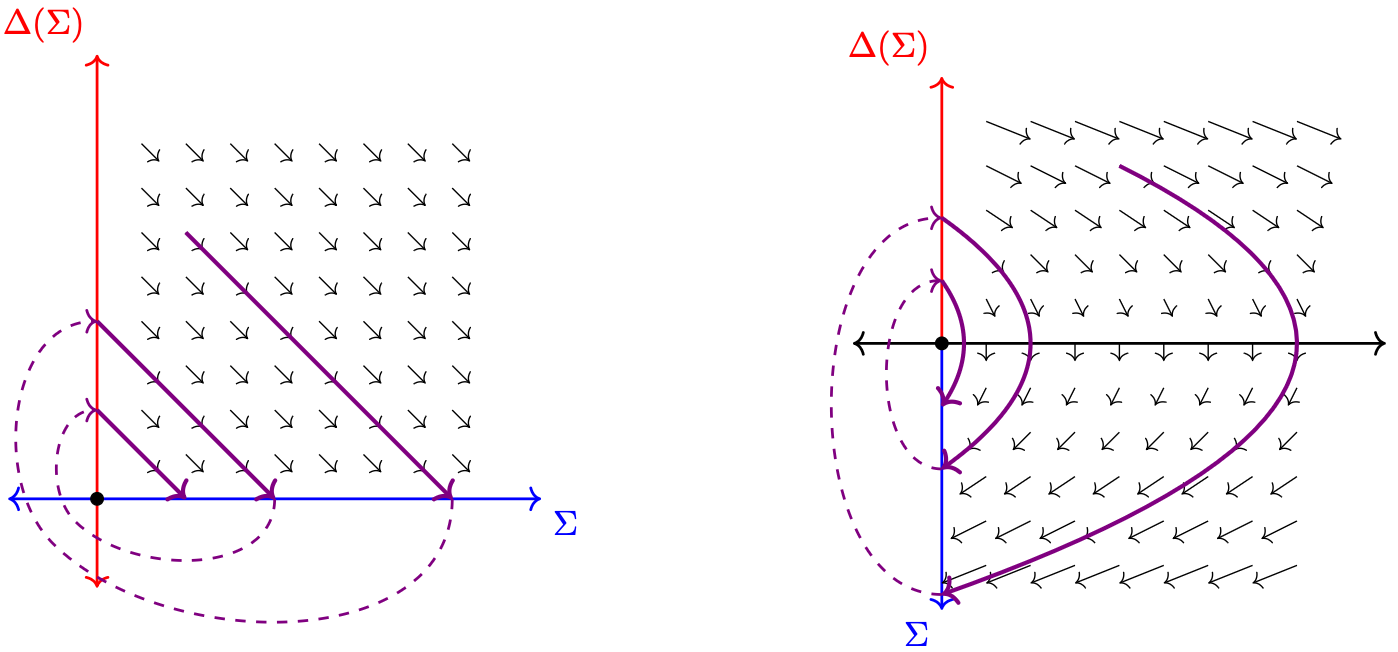
\includegraphics[width=0.7\textwidth]{./figures/linear-006.png}
    \caption{Two qualitatively distinct types of Zeno behaviors in planar affine hybrid systems~\cite{clark_linear}}
\end{figure}


\subsection{Hybrid Conley Index Theory (Kalies, Mischaikow)}\label{sec:hybrid_Conley}

The Conley index theory is a topological framework developed to capture the global structure of dynamical systems, especially when classical analytical tools fail.
It provides algebraic invariants—typically in the form of homology groups or pointed topological spaces—that classify isolated invariant sets and their dynamics.
These invariants are robust under perturbations and offer insight into complex behaviors such as recurrent dynamics, chaos, or bifurcations, even when explicit solutions are inaccessible.
In smooth dynamical systems, the Conley index unifies and extends results from Morse theory, fixed point theory, and symbolic dynamics.

\paragraph{Accomplishments}
In the setting of hybrid dynamical systems, the motivation to develop a Conley index theory stems from the challenges introduced by discontinuities and mode-switching, which obstruct the direct application of smooth analytical methods.
Standard techniques for constructing combinatorial models (e.g., cubical or simplicial complexes) and associating them with open classes of continuous dynamical systems do not directly extend to hybrid systems due to the absence of a globally defined flow or semiflow.
Nonetheless, understanding the global geometry and topology of hybrid state spaces—including attractor structure and invariant sets—remains a fundamental goal.
Conley index theory offers a promising route to extract robust, computable topological invariants that describe hybrid dynamics in a coordinate-free and discretization-friendly manner.

In \cite{KaRi-hybridCIT}, we introduced a combinatorial-topological framework for analyzing hybrid dynamical systems through an adaptation of Conley index theory.
We showed that, under suitable conditions, one can factor the hybrid dynamics through an associated semiflow whose structure reflects the original hybrid system.
This construction enables the use of reconstruction theorems and existing computational software to derive meaningful algebraic invariants from the hybrid system.
Importantly, the method extends to cases where the hybrid system does not satisfy the trapping guard condition, although in such cases the dynamical interpretation of the resulting invariants becomes more nuanced.
This work provides a computational pipeline that links hybrid dynamics to algebraic topology in a rigorous, extensible framework.

\paragraph{Future Directions}
We are currently working to extend this approach to broader classes of hybrid systems, especially in connection with the developments in \Cref{sec:learning_Mischaikow,sec:homologicaldynamicsHS,sec:DSGRN}.
This includes efforts to generalize the mathematical theory to cover more complex hybrid models, clarify the interpretation of algebraic invariants in the absence of standard dynamical conditions, and integrate these tools with the combinatorial-geometric perspectives developed elsewhere.
A key direction is to understand how to reconstruct or infer meaningful dynamics—such as attractors, invariant manifolds, and recurrence structures—from the topological data produced by the Conley index in hybrid contexts.

\begin{figure}
    \centering
    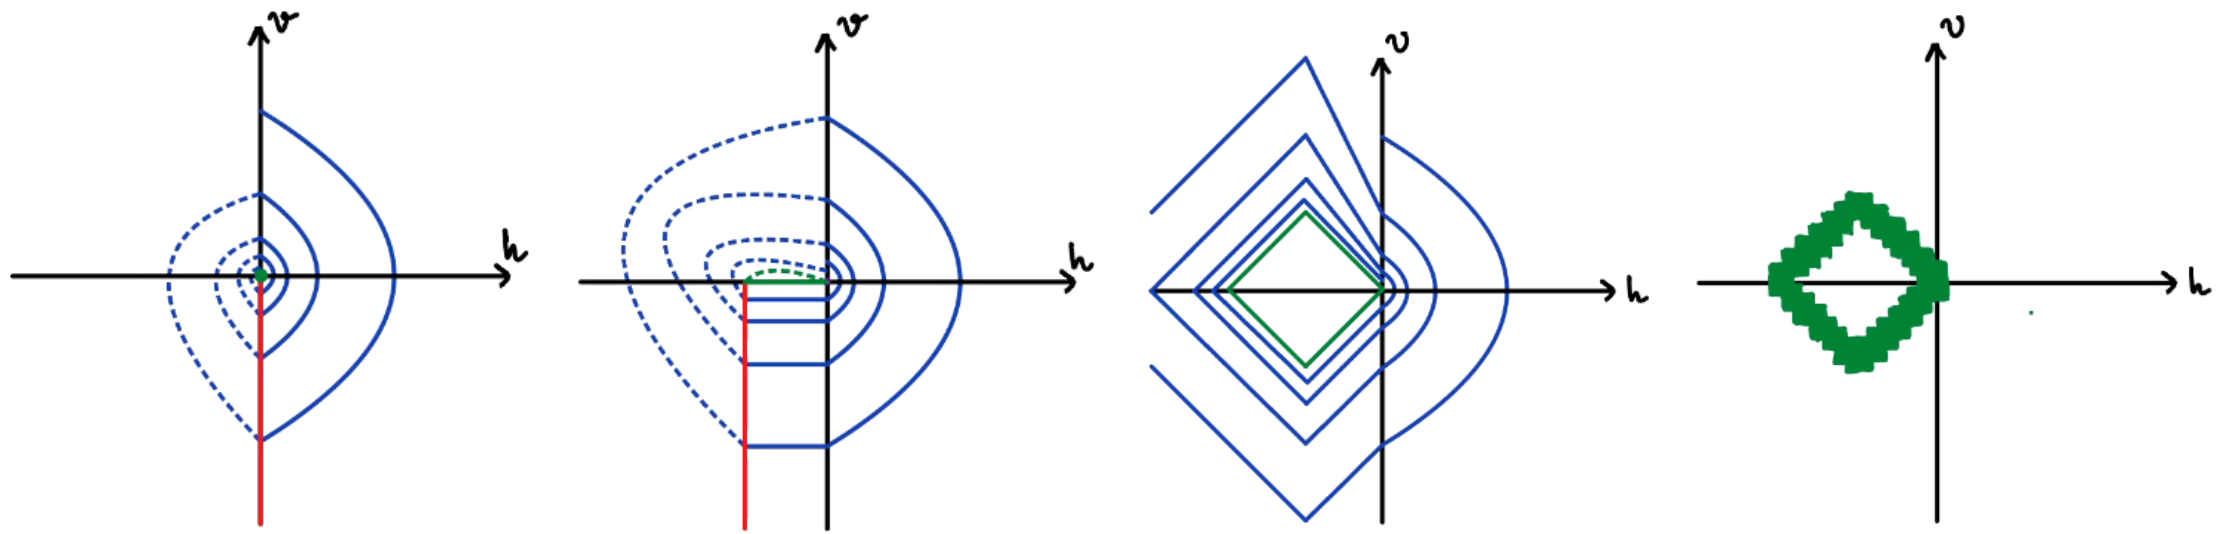
\includegraphics[width=0.9\textwidth]{./figures/bouncing_ball_Conley.png}
    \caption{Bouncing ball: from the phase portrait of the hybrid system to a combinatorial model~\cite{KaRi-hybridCIT}}
\end{figure}


%TL: any pre-print for [12]

\subsection{Homological Dynamics of Hybrid System (Mischaikow, Guralnik, Kalies)}
\label{sec:homologicaldynamicsHS}

Homological dynamics extends the ideas of Conley index theory to offer a global, algebraic-topological framework for understanding the structure of dynamical systems.
While Conley theory provides robust invariants for isolated invariant sets, homological dynamics seeks to organize and relate multiple invariant structures—such as attractors, repellers, and connecting orbits—into a coherent topological picture.
This is especially important for hybrid systems, where discontinuities and mode switches disrupt the applicability of smooth analytical tools and complicate the identification of classical invariant structures.
Homological dynamics, through constructions like attractor lattices and space-time decompositions, offers a flexible and computationally feasible approach to uncover system-wide behavior that is inaccessible to purely local methods.
This is particularly relevant in data-driven and computational settings, where hybrid systems often arise and where robustness to discontinuities is critical.

\paragraph{Accomplishments}

One concrete realization of these ideas is the Dynamical Systems Generated by Regulatory Networks (DSGRN) framework, which was developed to analyze the global dynamics of regulatory networks and hybrid systems involving discontinuous vector fields.
DSGRN replaces continuous ODE models with combinatorial dynamical systems derived from the system’s logical structure (e.g., thresholds, switches), using state-transition graphs to represent dynamics in a finite, discrete form.
This approach enables the identification of continuous dynamics consistent with appropriate regularizations—often implicit—of the original ODEs.
Through algebraic-topological constructions, DSGRN allows for rigorous dynamical analysis without requiring closed-form expressions for the regularized system.
The mathematical foundations of this method are detailed in \cite{gameiro2024globaldynamicsordinarydifferential}, with experimental validation in \cite{kepley2024globalanalysisregulatorynetwork}.
These results demonstrate how discrete representations of phase space and combinatorial models of dynamics can recover meaningful, robust invariants even in nonsmooth settings.

Our goal is to extend the DSGRN framework and philosophy to broader classes of hybrid systems.
We view hybrid dynamics as fundamentally multiscale, and while their models often include discontinuities, the underlying physical systems evolve continuously.
Our approach is to develop a topological and order-theoretic framework that provides a rigorous global characterization of hybrid system dynamics, without requiring explicit modeling of the physics at the discontinuities.
The main challenge lies in the fact that algebraic-topological invariants typically assume continuity.
To overcome this, we adapt the DSGRN two-step process:
(i) constructing a discrete phase space rich enough to resolve discontinuities, and
(ii) building a combinatorial model of dynamics compatible with the appropriate regularized continuous system.
For complex hybrid systems, both components may need to be adapted to capture system-specific features.

\paragraph{Future Directions}

A recent development in this direction is presented in \cite{ClGu-weakened_topologies}, where we introduce a procedure that associates a weakened $T_0$ topology to hybrid state spaces via their jump (reset) relations.
In this weakened topology, hybrid trajectories—including those accumulating on guards without intersecting them transversely—become continuous functions of time.
This approach broadens the allowable types of discontinuities while avoiding the need for artificial state identifications or hybrid time domains.
Inspired by the paradigm of homological dynamics, where cellular spaces are represented up to weak homotopy equivalence by their $T_0$ quotients, we aim to develop a topological framework for hybrid systems where dynamics are described via multivalued maps or multivector fields over topologically regularized spaces.
This extension will provide a principled way to analyze hybrid systems using algebraic-topological tools, consistent with the homological and Conley-based perspectives introduced in Section~\ref{sec:hybrid_Conley}.

%TL: any write-up for \cite{ClGu-weakened_topologies}?

\subsection{Data-Driven Topological Analysis of Hybrid Systems (Mischaikow, Clark, Kalies)}\label{sec:learning_Mischaikow}

The analysis of nonlinear dynamical systems is undergoing a paradigm shift toward data-driven methods, motivated by the growing availability of large-scale data and recent advances in machine learning.
Traditional modeling techniques—whether based on parametric differential equations or black-box surrogate models—often lack robustness in capturing long-term behaviors, particularly near bifurcations.
In contrast, Conley index theory offers a topological framework for extracting robust, global information about a system’s dynamics, including the existence and structure of invariant sets and attractors.
The central goal is to integrate machine learning with Conley index theory to infer qualitative features of complex dynamical systems directly from data, without requiring explicit equations.
This integration allows for the automated identification of regions of interest (e.g., basins of attraction) and computation of topological invariants using learned discretizations of phase space.
Such a framework is both scalable and interpretable, offering a promising direction for analyzing high-dimensional, nonlinear, or data-defined systems.

\paragraph{Accomplishments}

In \cite{gameiro2025rigorouslycharacterizingdynamicsmachine}, we argue that the classical approach to nonlinear dynamics—based on detailed invariant structure—is too rich to be fully recovered from data.
Instead, we show that dynamics characterized via order theory and algebraic topology, particularly through Conley index theory, can be learned given sufficient data and computational resources.
Further, in \cite{gameiro2025datadrivenidentificationattractorsusing}, we explore the use of machine learning to identify attracting regions using orbit-labeled data from known ODEs.
By learning an appropriate discretization of phase space (typically a compact hyper-rectangle in $\mathbb{R}^n$), we approximate attracting neighborhoods whose topological invariants match those of known attractors, thereby validating the approach.
We also demonstrate that, when using networks constrained to produce cubical decompositions (e.g., via linear transformations of parallelotopes), computational homology (e.g., via \texttt{pyCHomP}) becomes tractable.
Though such networks limit the geometric complexity that can be represented, test examples confirm that correct Conley indices can still be obtained, as long as the network accurately approximates the labeling function.
Additionally, we propose heuristics to detect whether a given network architecture is sufficient to capture complex basin geometries.

\begin{wrapfigure}[11]{r}{0.4\textwidth}
    \centering
    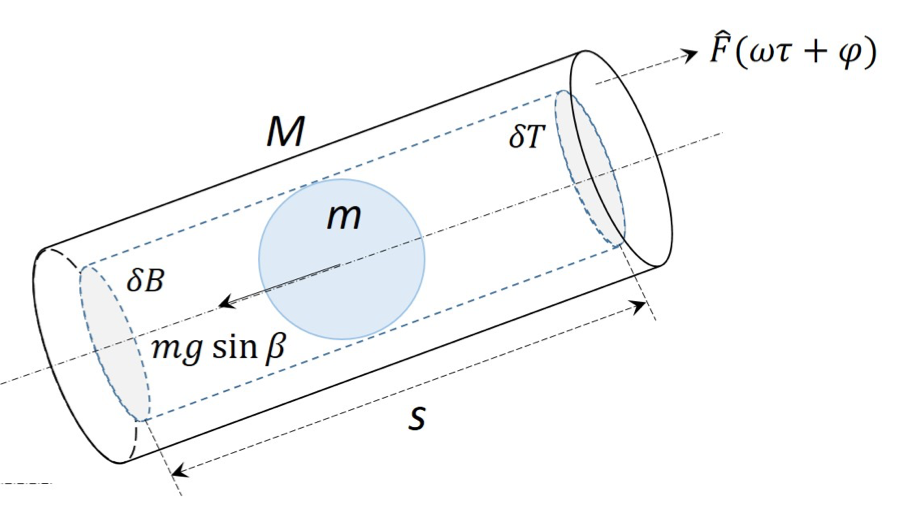
\includegraphics[width=0.4\textwidth]{figures/vibro-impact.png}
    \caption{Vibro-impact energy harvester}
\end{wrapfigure}
Based on these exploratory studies, we have begun the process of extending these ideas to the setting of hybrid systems. 
In particular, in joint work with Kuske (GaTech) we have been developing computational tools to characterize the global dynamics of a vibro-impact energy harvester (see \cite{serdukova2021post}), 
which is a mechanical system that converts ambient vibrations into electrical energy by using mechanical impacts between a vibrating structure and physical stops. These impacts introduce nonlinear dynamics that broaden the frequency range and enhance energy output compared to traditional resonant harvesters. While they offer improved performance in variable or broadband vibration environments, they also pose challenges such as mechanical wear and complex modeling.
Our code is now capable of characterizing the lattice of attractors even though the  phase space for the data provided by R. Kuske lies on a manifold as opposed to Euclidean space.
More specifically, using data coming from simulations provided by Kuske we are attempting to characterize lattices of attractors and compute Conley indices. 

\paragraph{Future Directions}

A fundamental challenge is to develop a computational Conley index theory that is capable of characterizing dynamics even though hybrid systems exhibit discontinuous dynamics.
As is argued in Section~\ref{sec:homologicaldynamicsHS} we have achieved this in the context of DSGRN where the goal is to characterize the dynamics of a ODE.
However, in the data-driven setting it is more natural to assume that we are trying to characterize the dynamics induced by a map.
In this context it appears that discontinuities range from ignorable to local to global. 
As of yet these terms are not defined, but the intuition is as follows.
We are using a cellular theory of homological computations, thus discontinuities that fall within individual cells have no impact on the homological computations and can be easily regularized.
Local discontinuities lead to non-acyclic images -- on a technical level this violates the acyclic carrier theorem that is often used to prove that maps induced by homology are well-defined.
Earlier work by Mischaikow and co-authors suggests possibilities for addressing this setting.
Global discontinuities are a wide open challenge.
In summary we need to define these terms, develop algorithms for identifying these settings, and develop mathematical theory that leads to proper regularizations. 


\subsection{Nonholonomic Mechanical Hybrid Systems and Control (Bloch, Clark)}\label{sec:nonholomomic}

Nonholonomic mechanical systems--those with non-integrable velocity constraints--arise naturally in robotics, locomotion, and mechanical design. 
When such systems experience impacts (e.g., collisions with surfaces or between bodies), the dynamics become hybrid, combining smooth evolution governed by differential equations with discrete events marked by abrupt velocity changes. 
Modeling these systems accurately is challenging, as traditional variational approaches break down in the presence of nonholonomic constraints. 
Understanding the post-impact dynamics, particularly under nonholonomic constraints, is essential for designing stable locomotion strategies, developing energy-efficient mechanical systems, and extending optimal control principles to hybrid domains. 

\paragraph{Accomplishments}

In prior work \cite{clark2019bouncing}, we studied the dynamics of a rolling disk undergoing collisions with convex barriers—such as circles or ellipses—extending classical billiard dynamics to the nonholonomic setting. 
This setup, referred to as the bouncing penny, illustrates the hybrid nature of mechanical systems subject to rolling constraints and impacts. 
The key innovation was the derivation of nonholonomic impact laws using an analogue of the Weierstrass-Erdmann corner conditions, which in classical Lagrangian systems describe variational impacts. 
Since nonholonomic systems are not strictly variational, the analysis required reformulating the problem using the Lagrange-d’Alembert principle and viewing the nonholonomic dynamics as projections of variational flows. 
This approach clarified how discontinuous transitions (impacts) interact with continuous rolling constraints and provided a rigorous geometric framework for simulating and analyzing such systems.
Further, these systems are also motivated from a control-theoretic perspective, as they can emerge from Pontryagin’s maximum principle applied to hybrid control problems with mechanical structure \cite{clark_oc}.

\paragraph{Future Directions}

We are currently extending this framework to a broader class of nonholonomic systems with impacts, including classical models such as the Chaplygin sleigh. 
Our goal is to analyze the integrability, energy behavior, and geometric structure of these systems when subjected to collisions. 
Additionally, we are studying the role of external forces—particularly gravity—and considering both elastic and inelastic impacts. 
A key focus is the stability of contact equilibria, where the system may come to rest or repeatedly impact a surface. 
We aim to generalize classical stability results from holonomic systems to nonholonomic and hybrid settings, providing new insights into the long-term behavior of mechanical systems with impacts. 
This work will also inform the development of hybrid control strategies for nonholonomic mechanical systems.

%This work builds on our previous work on the dynamics  of mechanical systems with collisions. 
%We consider both Hamiltonian and nonholonomic systems and collisions with various barriers as well as collisions between objects. 
%In past work \cite{clark2019bouncing}, we considered the dynamics of a rolling disk colliding with a convex barrier such a circle or ellipse generalizing standard work on billiard collisions. 
%Also, these types of systems arise from Pontryagin's maximum principle for a general class of hybrid dynamical systems (\cite{clark_oc}). 
%We are generalizing this to the dynamics of other nonholonomic systems such as the Chaplygin sleigh and analyzing integrability. 
%In addition we are analyzing the dynamics of systems under gravitational forces and examining  elastic and inelastic collisions as well as the stability of the resulting contact equilibria. 
%This will generalize classical results on the stability of contact equilibria to the dynamics setting. 

\subsection{Hybrid Holonomy (Guralnik, Clark)}\label{sec:holonomy}

Holonomy refers to the phenomenon where periodic changes in internal (shape) variables of a system produce non-periodic changes in external (group) variables—as observed in locomotion. 
For instance, during bipedal walking, the legs follow a periodic gait, yet the body progresses forward. 
This geometric insight motivates the use of principal bundles in modeling locomotion, where the system’s configuration space is decomposed into shape variables (internal) and group variables (external). 
A connection on the principal bundle couples these variables, and the holonomy group captures the net motion in the external space induced by loops in the shape space. 
If the connection is flat, no net motion is possible, and the holonomy group is trivial.

However, in many practical systems with intermittent contact or impact dynamics—such as walking, hopping, or manipulation—the system undergoes non-smooth transitions between phases. 
These transitions enable behaviors that would be impossible for the individual smooth components. 
For example, walking can be modeled as a sequence of inverted pendulum arcs, each incapable of producing net motion, but together yielding forward propulsion. 
This richer behavior motivates the development of a hybrid extension of the principal bundle framework, which we term a hybrid principal bundle.

\paragraph{Accomplishments}

A major challenge in extending holonomy to hybrid systems is that concatenating flat connections across discrete transitions does not necessarily preserve flatness. 
In legged locomotion, for example, each individual stance phase may correspond to flat dynamics, yet their sequential composition yields non-zero holonomy. 
Formally defining holonomy in this non-smooth setting requires a framework that can consistently account for phase-dependent transitions, impacts, and resets. 
A further difficulty lies in ensuring the holonomy group remains well-defined under hybrid dynamics—particularly when guards (reset surfaces) and resets are defined via constraints on the shape space.

\begin{wrapfigure}[13]{r}{0.4\textwidth}
    \centering
    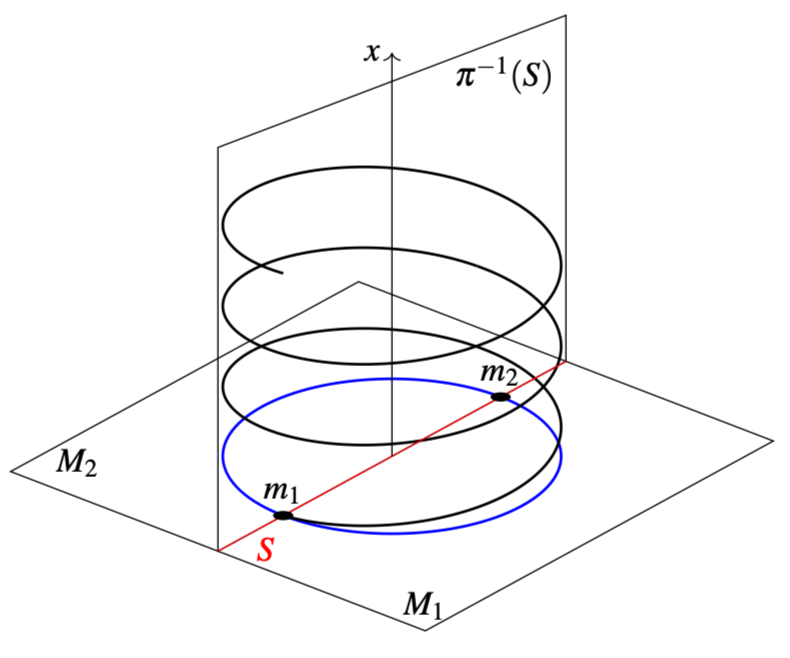
\includegraphics[width=0.35\textwidth]{./figures/hybrid_holonomy.png}
    \caption{Hybrid bundle with two component $M_1$, $M_2$, and impact surface $S$}
\end{wrapfigure}
In recent work \cite{hybrid_holonomy}, we developed a formal framework for defining and computing the holonomy group of hybrid systems, and analyzed their behavior in the limit as the number of impacts increases. 
We showed that if the guards are defined on the shape space, then the hybrid holonomy group is well-defined. 
Additionally, we observed that piecewise-flat trajectories—such as those in hybrid locomotion—can be approximated by smooth curved trajectories. 
For example, walking can be viewed as an approximation to rolling, and the peg-in-a-slot problem can be approximated by the dynamics of the Chaplygin sleigh. 
This suggests a close relationship between hybrid principal bundles with flat components and smooth principal bundles with curved connections, linked via suitable metric limits.

\paragraph{Future Directions}

We aim to rigorously formalize this relationship using the language of metric limits, in which a curved principal bundle arises as the limit of hybrid bundles composed of flat elements. 
A central challenge is to develop a systematic method to decompose an arbitrary shape space into components that allow this limiting procedure. 
To that end, we seek a broad generalization of the notion of a hybrid bundle that can incorporate arbitrarily fine open covers of the shape space, consistent with the evolving topological framework outlined in Section~\ref{sec:homologicaldynamicsHS}.
This would enable hybrid holonomy theory to be applied to general hybrid systems and would provide a unified geometric framework for locomotion, manipulation, and other impact-driven behaviors.


%A system with intermittent contact/impacts can achieve richer motion than its constituent components can, e.g. bipedal locomotion can be achieved as a sequence of inverted pendulums while the later is incapable of locomotion. 
%This motivates the concept of a \textit{hybrid principal bundle}.

%A principal bundle is a space which consists of internal (shape) and external (structure group) variables. 
%The shape and group variables are coupled through a choice of a connection on the bundle. 
%This offers a convenient framework for studying locomotion as the set of possible net changes in the external variables are achievable from periodic motions in the shape variables (holonomy group) by imposing the constraints from the specified connection. 
%When no net change in the group variables is achievable (the holonomy group is trivial), the connection is called \textit{flat}.

%As seen with legged locomotion, non-smooth concatenation of flat connections need not remain flat (as walking comprised of multiple steps). 
%This observation may be case in the framework of hybrid principal bundles, where we have shown that the holonomy group is well-defined provided the guards are defined by constraints on the shape space. 
%Moreover, piece-wise flat trajectories can be well-approximated by curved ones, e.g., walking by rolling and a peg-in-a-slot by the Chaplygin sleigh \cite{hybrid_holonomy}. 
%More formally, we aim to express this observation in terms of metric limits, where the curved principal bundle is the limit of hybrid principal bundles (with flat components). 
%A major challenge is to determine a systemic way to decompose an arbitrary shape space such that the metric limit may be applied. 
%A broad formulation of the notion of a hybrid bundle is required that would enable the use of arbitrarily fine open covers of the shape space and the study of the associated limits. Such a formulation would be an extension of the topological hybrid framework being developed under Section~\ref{sec:homologicaldynamicsHS}.

% \dg{A system with intermittent contact/impacts can achieve richer motion than its constituent components can, e.g. bipedal locomotion can be achieved as a sequence of inverted pendulums while the latter is incapable of locomotion.
% This motivates the concept of a \textit{hybrid principal bundle}.}

% \dg{A principal bundle is a space which consists of internal (shape) and external (structure group) variables. The shape and group variables are coupled through a choice of a connection on the bundle.
% This offers a convenient framework for studying locomotion as the set of possible net changes in group variables achievable from periodic motions of the shape variables (holonomy group), subject to the constraints imposed by the specified connection.
% When no net change in the group variables is achievable through shape changes (the holonomy group is trivial), the connection is referred to as \textit{flat}.}

% \dg{
% As seen with legged locomotion, non-smooth concatenation of flat connections need not remain flat.
% This observation may be cast in the framework of hybrid principal bundles, where we have shown that the holonomy group is well-defined provided the guards are defined by constraints set on the shape space.
% Moreover, a hybrid principal bundle with flat components can be well-approximated by a curved bundle, e.g. walking by rolling and a peg-in-a-slot by the Chaplygin sleigh.
% (WILL, IS THERE ANYTHING MORE WE WOULD LIKE TO SAY AS FAR AS ACHIEVEMENTS GO? \cite{hybrid_holonomy})
% More formally, we aim to express this observation in terms of metric limits, where the curved principal bundle is the limit of hybrid principal bundles with flat components, as the flat components are compressed indefinitely in the sense of the diameters of their bases being shrunk to zero.
% A major challenge is that is may be impossible to decompose an arbitrary shape space into arbitrarily small polyhedra (the polyhedral structure corresponding to impacts).
% Instead, a broader formulation of the notion of hybrid bundle is required that would enable the use of arbitrarily fine open covers of the shape space and the study of the associated limits.
% Such a formulation would also need to be consistent with the more general hybrid systems framework being developed under Section~\ref{sec:homologicaldynamicsHS}.}

\section{Openness and Composition}\label{sec:OC}

The research theme of Openness and Composition addresses fundamental challenges in modeling, analyzing, and controlling hybrid systems interacting with uncertain environments and dynamic network structures. 
This includes the development of Lyapunov-based methods for ensuring stability in switching and heterogeneous hybrid dynamic networks, with extensions to topological analysis via DSGRN (\Cref{sec:dynamic networks in DSGRN}). 
To handle uncertainty in hybrid systems, transfer operator methods were introduced for stochastic hybrid systems, enabling operator-theoretic characterization of their global statistical behavior (\Cref{sec:SHS}). 
Complementary work on stochastic mechanical systems has produced structure-preserving integrators that accurately capture the energetic and statistical properties of systems with impacts (\Cref{sec:geo_int}). 
In the absence of reliable probabilistic models, deterministic uncertainty frameworks were developed to ensure conservative and robust control based on bounded state estimation (\Cref{sec:deterministic_uncertainty}). 
Finally, a generalized metriplectic framework integrates dissipative effects into geometric mechanics, allowing the identification of thermodynamically consistent models from data (\Cref{sec:metriplectic}). 
Together, these efforts advance the theoretical foundations and computational tools for scalable analysis and control of open, uncertain, and interconnected hybrid systems.

\subsection{Hybrid Dynamic Networks (Bloch, Mischaikow, Kalies, Guralnik)}\label{sec:dynamic networks in DSGRN}

Network dynamical systems—comprising interconnected nodes with local dynamics influenced by neighboring interactions—are fundamental models in areas such as communication networks, biological regulation, and power grids. 
A critical issue in such systems is stability, which can be compromised by the inherent nonlinearity and complex inter-node coupling. 
While appropriately designed coupling strategies can promote synchronization and enhance global stability, poorly structured coupling can destabilize the entire system—even if individual node dynamics are stable.
The challenge intensifies when the coupling structure itself changes over time, a phenomenon known as switching. 
Such switching is common in real-world applications, where the connectivity of a network may be altered due to external inputs, system constraints, or failures. 
These structural changes can significantly impact stability, motivating the need for a rigorous theoretical framework that ensures robustness under arbitrary switching of coupling structures.

\paragraph{Accomplishments \& Directions}

We developed a Lyapunov-based framework to analyze the stability and stabilization of diffusively coupled dynamical systems, with a focus on networks undergoing time-varying (switched) interconnections. 
We derived explicit expressions for critical coupling parameter values that govern whether the entire system remains stable, even when individual nodes exhibit unstable dynamics. 
In addition, we established sufficient conditions for ensuring asymptotic stability under arbitrary switching in the network topology or coupling strength. 
These results are supported by numerical simulations that confirm the accuracy and practical relevance of the theoretical findings \cite{mouyebe2025coupling}.  

We are currently extending these ideas to hypergraph networks both with linear and nonlinear coupling, see e.g \cite{pickard2024kronecker}. 
We aim to extend these results to heterogeneous networks with diverse node dynamics and to incorporate delays and nonlinear coupling terms, which are prevalent in real-world systems. 
Another important direction is to investigate distributed control and optimization methods that allow real-time adjustment of coupling to preserve stability under constraints. 
Finally, we plan to explore applications to critical infrastructure systems, such as smart grids and multi-agent robotic systems, where coupling-induced stabilization is essential for resilience and performance in the presence of structural variability and external disturbances.

We are also applying these ideas to large data sets and to hybrid vector fields analyzed in the DSGRN framework discussed in \Cref{sec:homologicaldynamicsHS},
where we will study coupled network dynamics from a homological perspective.
We plan to extend the theoretical framework in DSGRN (\cite{gameiro2024globaldynamicsordinarydifferential}) to recast the problem of changes in network topology as changes in parameters of a larger network.
This allows one to characterize the global dynamics of switching networks by constructing combinatorial models that preserve algebraic topological invariants across different network configurations.
This approach will enable us to systematically analyze how network reconfiguration affects equilibria, periodic orbits, and connecting orbits, while identifying critical parameter regions where qualitative changes in system behavior occur.
%
%\dg{ALL, I am happy with this version as is, but I must still ask: would you like me to throw strategy spaces into the mix here? Thanks, --Dan. Tony: I would be okay if you added that. }

\begin{figure}
    \centering
    \subcaptionbox{Randomly selected set of non-positive divergence graphs}[0.45\textwidth]%
    {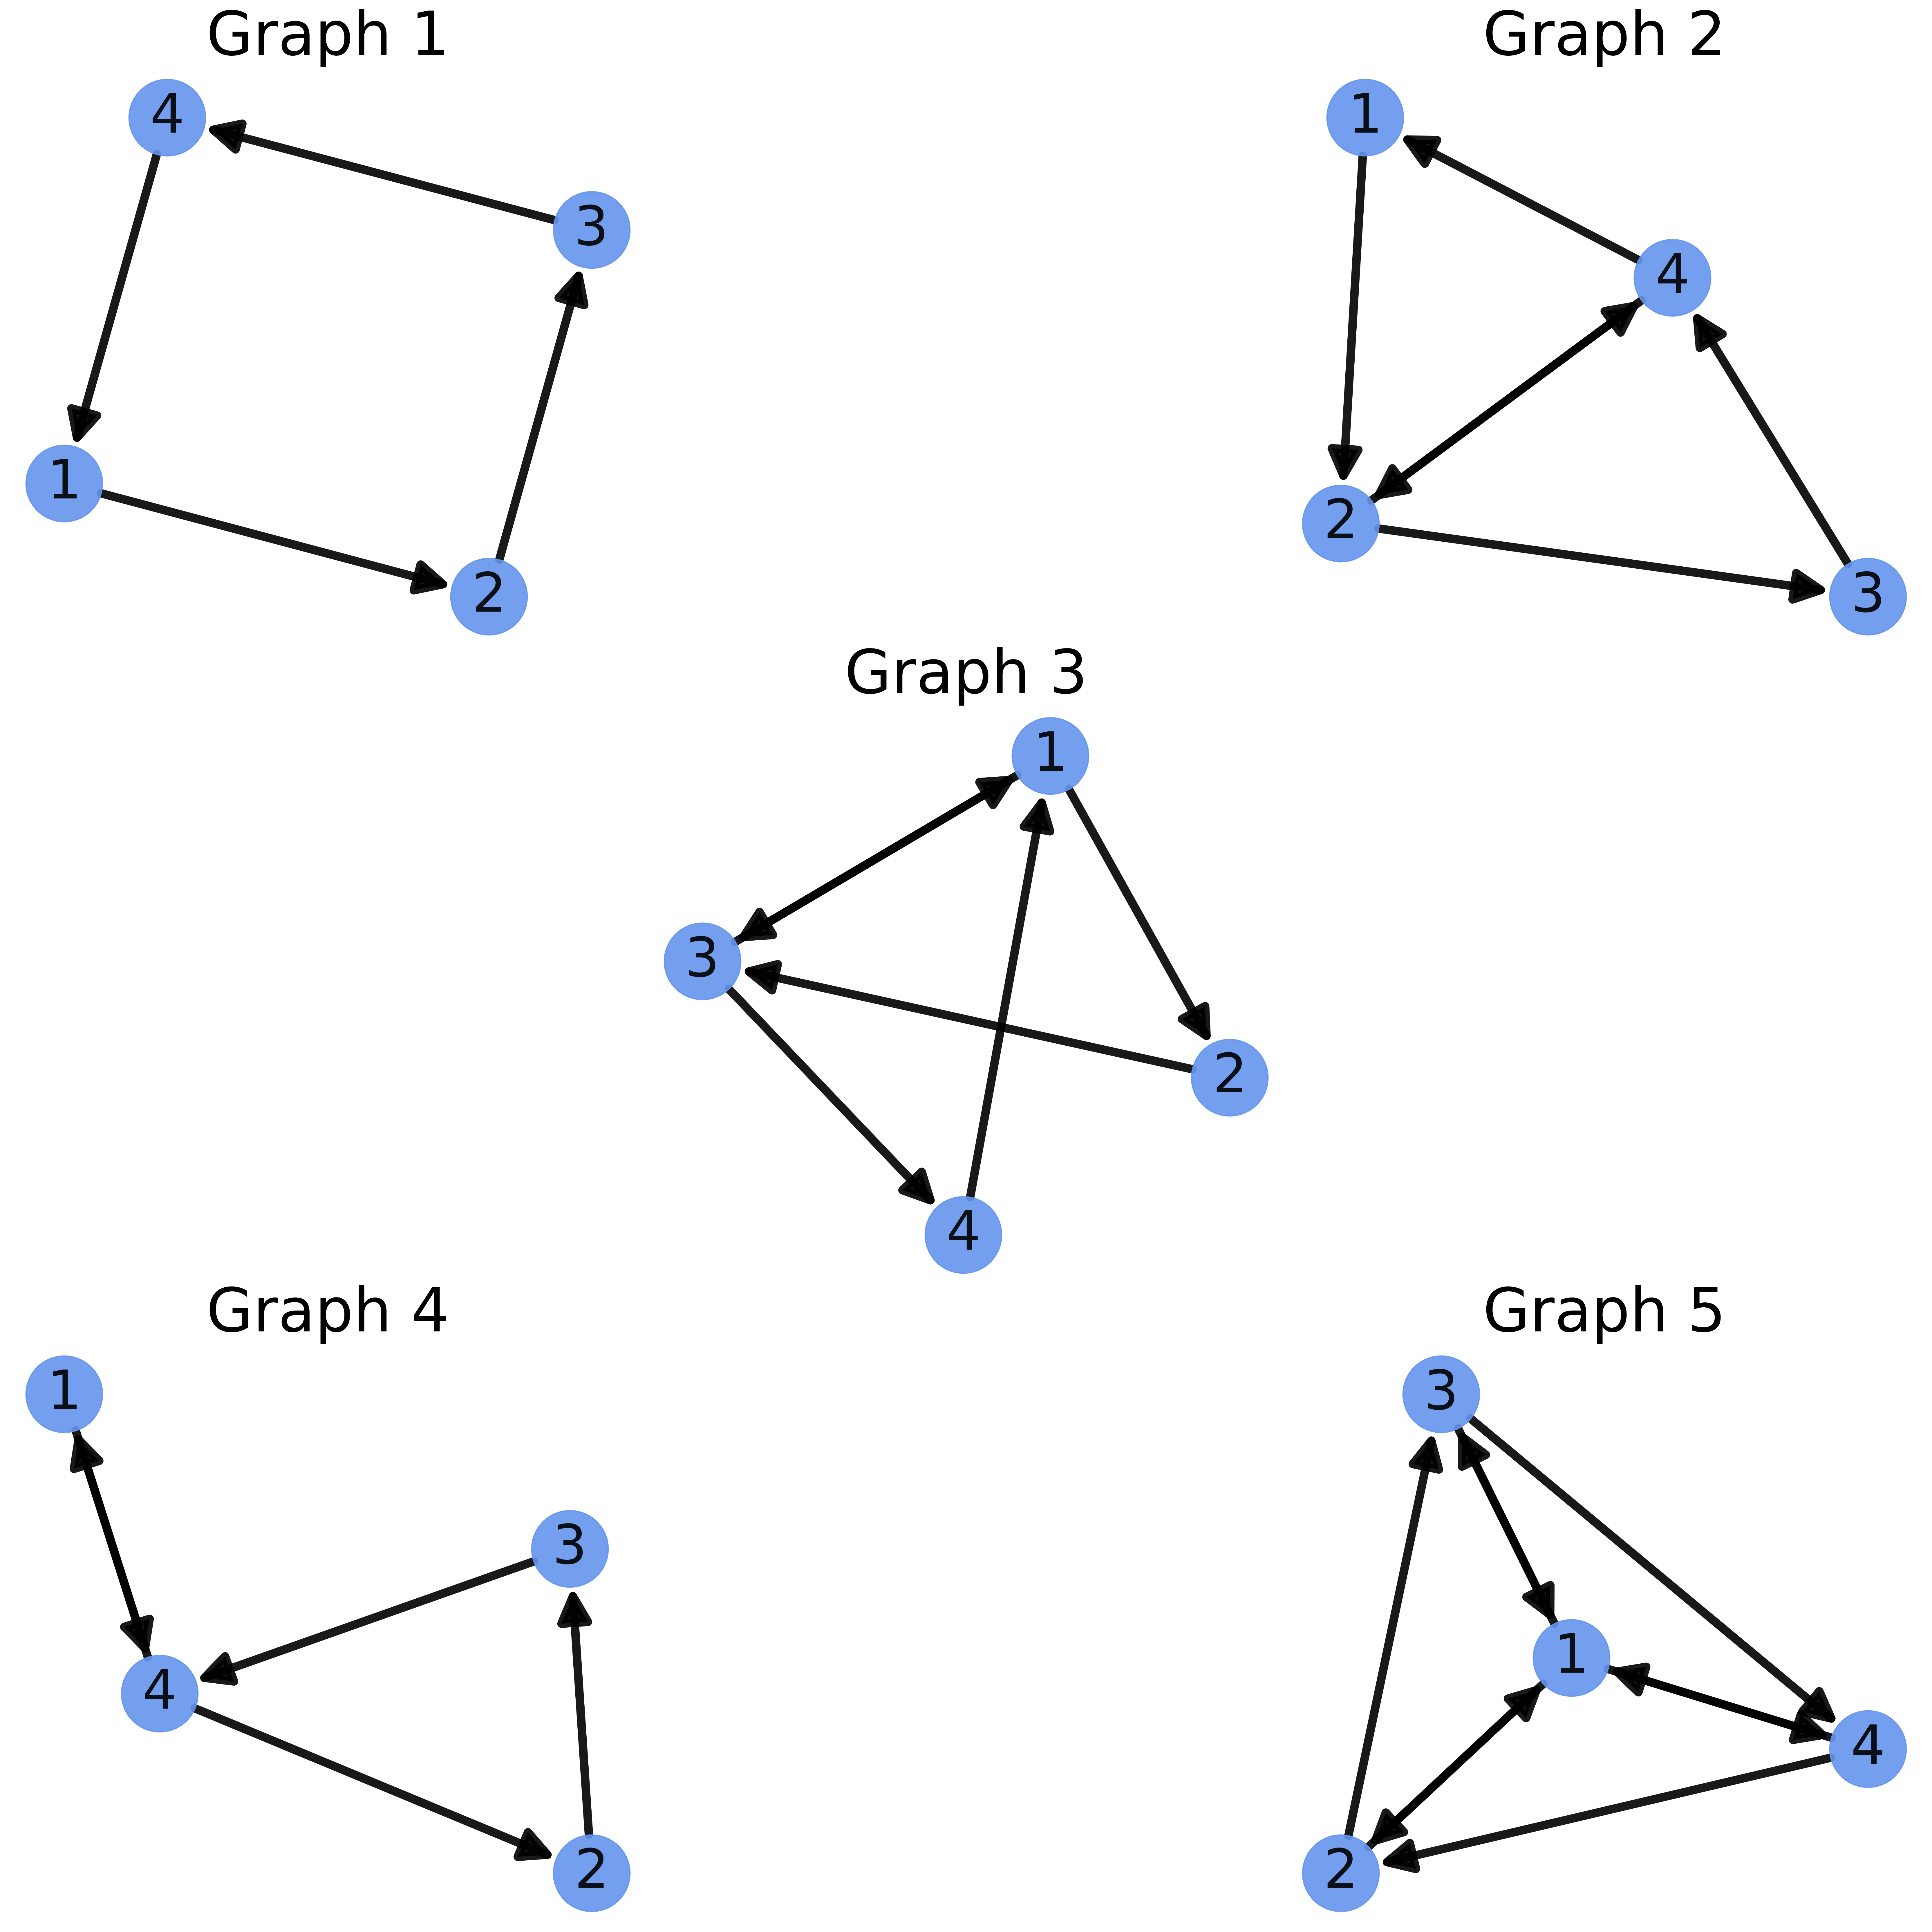
\includegraphics[height=0.2\textwidth]{figures/nds-008.png}}
    \hspace*{0.3cm}
    \subcaptionbox{Switched network system response over the network topologies}[0.45\textwidth]%
    {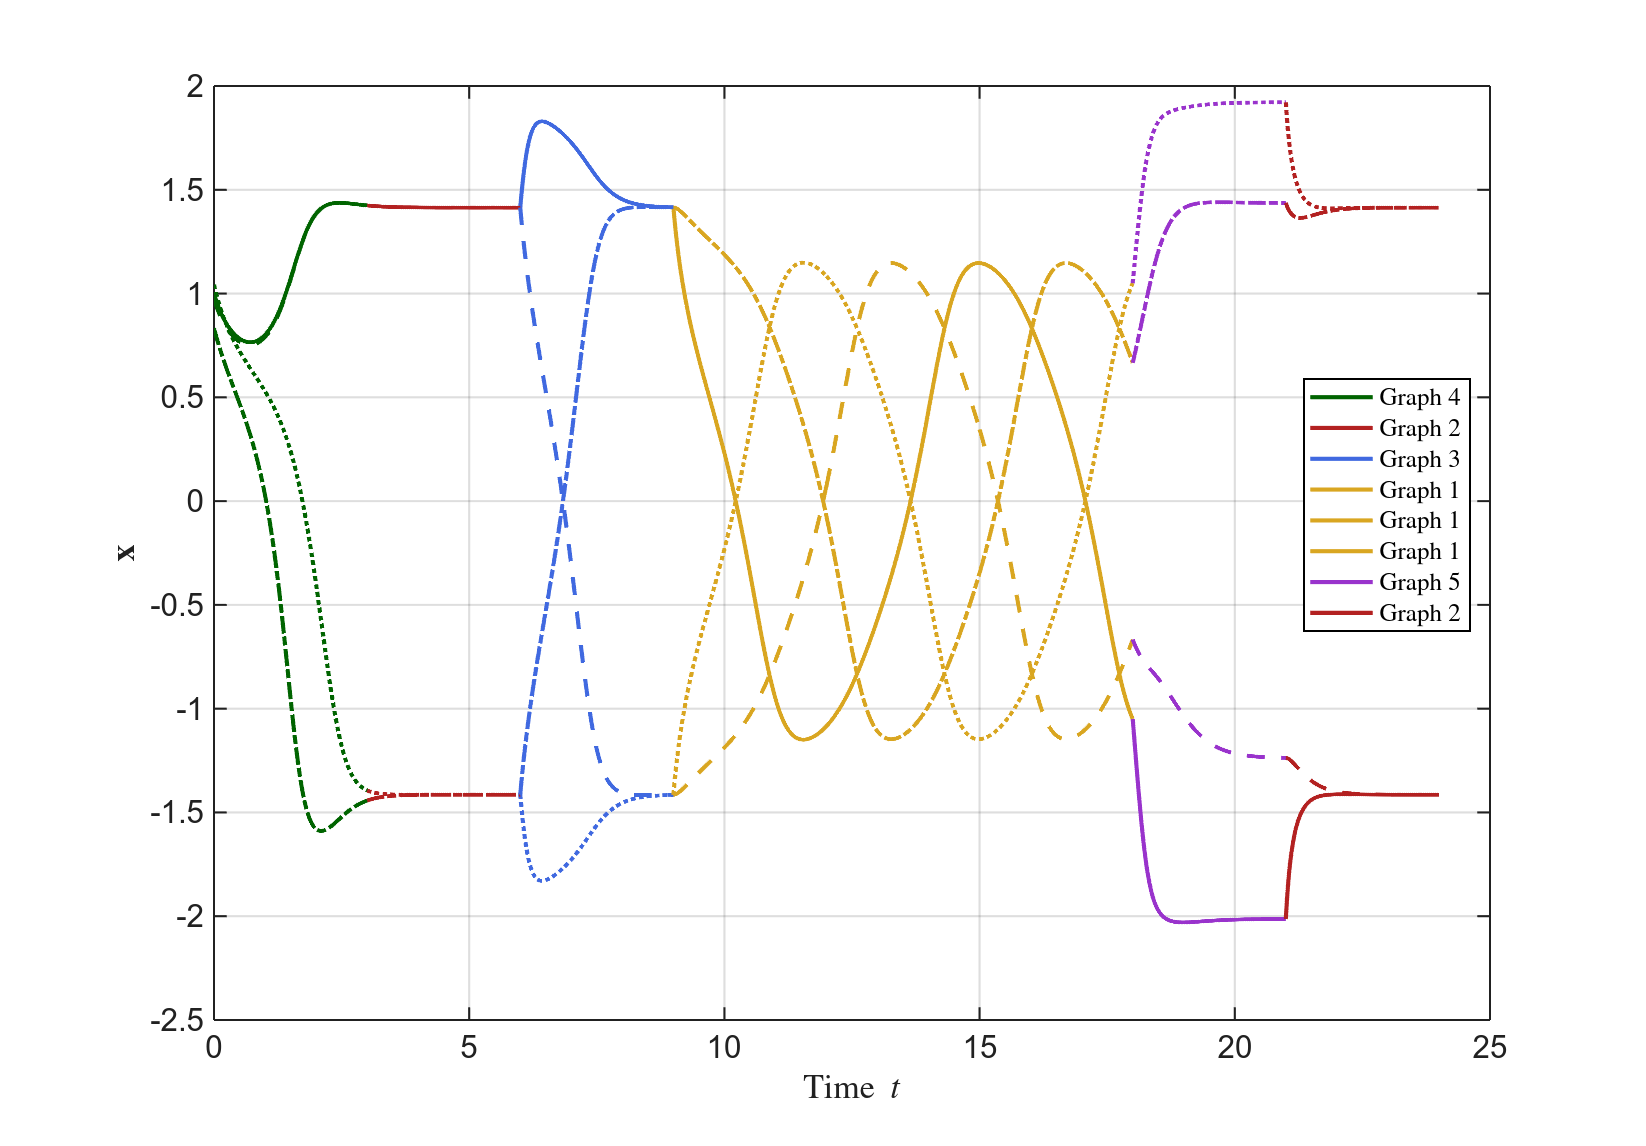
\includegraphics[height=0.2\textwidth]{figures/nds-010.png}}
    \caption{Hybrid dynamic network: coupling induced stabilization of network dynamical systems and switching~\cite{mouyebe2025coupling}}
\end{figure}

\subsection{Stochastic Hybrid System (Lee, Clark)}\label{sec:SHS}

A stochastic hybrid system (SHS) provides a comprehensive framework for modeling systems with uncertainties in both continuous and discrete dynamics.
The continuous state evolves according to stochastic differential equations tied to discrete modes, while discrete jumps are triggered either deterministically by entering guard sets or spontaneously via Poisson processes.
Post-jump states are determined by a stochastic kernel.
Thanks to its flexibility in incorporating uncertainty across all components, SHS has found wide application in fields such as robotics, biology, finance, and networked systems.

Analyzing SHS is challenging due to its combination of nonlinearity, discontinuities, and randomness.
To address this, a powerful approach is to shift from trajectory-based analysis to studying how distributions and observables evolve over time—formalized through transfer operators.
These operators capture the global dynamics of the system in a linear, though infinite-dimensional, framework.
The two primary operators are the Frobenius-Perron operator, which governs the evolution of probability densities, and the Koopman operator, which describes the evolution of observables (i.e., functions on the state space).
Despite the system’s underlying nonlinearity and stochasticity, these operators are linear, enabling the use of spectral and functional analytic tools.

\paragraph{Accomplishments \& Directions}

In this work, we formulated transfer operators for stochastic hybrid systems.
We derived their generators as partial differential equations reflecting the continuous dynamics, with boundary conditions induced by discrete events~\cite{stochastic-hybrid}.
This generalizes previous deterministic results, such as the hybrid Jacobian~\cite{OpSh_fp}, to stochastic settings.
We also analyzed how different types of jumps—guard-triggered vs. spontaneous—and various reset mechanisms (e.g., reflecting, absorbing, resetting) qualitatively affect system behavior.
These effects were verified through Monte Carlo simulations.

Hybrid transfer operators offer a rigorous framework for studying long-term statistical properties such as invariant measures, ergodicity, mixing, and metastability.
They are particularly valuable for revealing how randomness and switching interact to shape global behavior—phenomena often hidden from local or trajectory-based analyses.
Furthermore, this operator-theoretic perspective enables the development of data-driven methods (e.g., Dynamic Mode Decomposition, Ulam’s method) to approximate system dynamics directly from simulations or observations, making it both a theoretically robust and practically applicable tool for complex hybrid systems.
Our current efforts are focused on extending these results to higher-dimensional systems on a manifold.

%As hybrid systems are comprised of multiple interlocking components, stochasticity may be interpreted in many different ways. In \cite{stochastic-hybrid}, two stochastic cases are presented extending the deterministic results of \cite{OpSh_fp} to systems whose continuous dynamics are stochastic and discrete dynamics are either deterministic or stochastic. The Koopman operator encodes the expected value of an observable while the Frobenius-Perron operator is its adjoint and evolves densities. The generator for these operators is comprised as a partial differential equation (PDE) (arising from the continuous dynamics) and boundary conditions (arising from the discrete dynamics). The induced boundary conditions are qualitatively different depending on whether the jumps are stochastic or deterministic. Numerical experiments utilizing Monte Carlo simulation are performed to validate the analytic predictions from the hybrid PDE. We are extending these restults to higher dimensions and to general manifolds.


\begin{figure}
    \centering
    \subcaptionbox{Deterministic flow with forced jump}[0.32\textwidth]{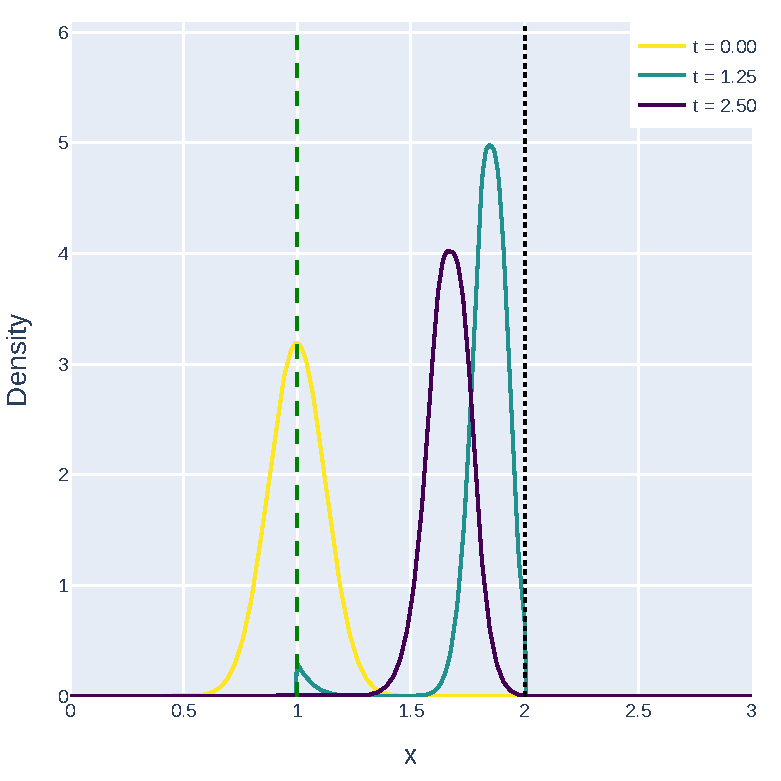
\includegraphics[height=0.25\textwidth]{figures/density_evolution_ideal_jump.pdf}}
    \subcaptionbox{Stochastic flow with forced jump}[0.32\textwidth]{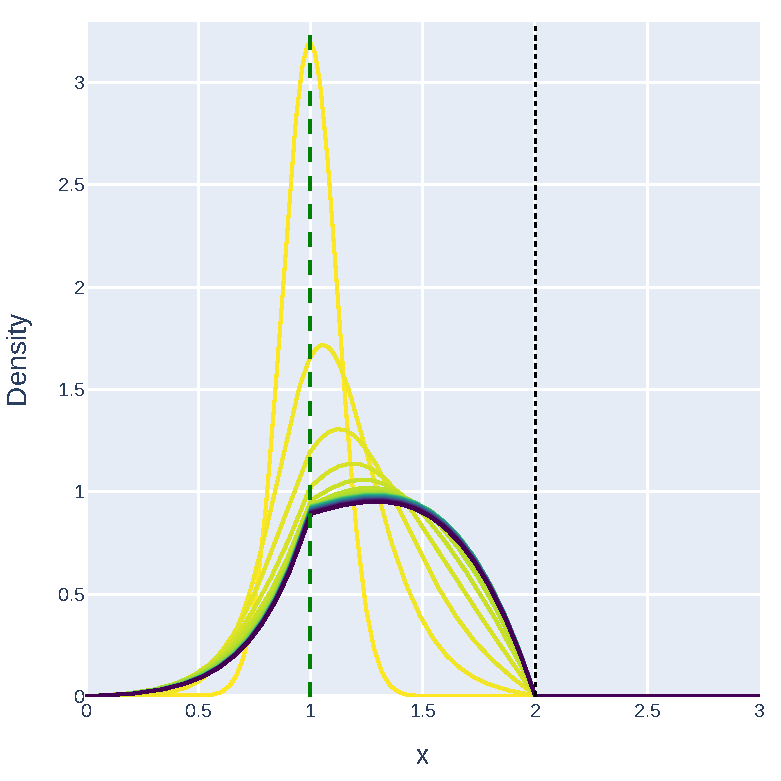
\includegraphics[height=0.25   \textwidth]{figures/density_evolution_det_jump_max_sigma.pdf}}
    \subcaptionbox{Stochastic flow with spontaneous jump}[0.32\textwidth]{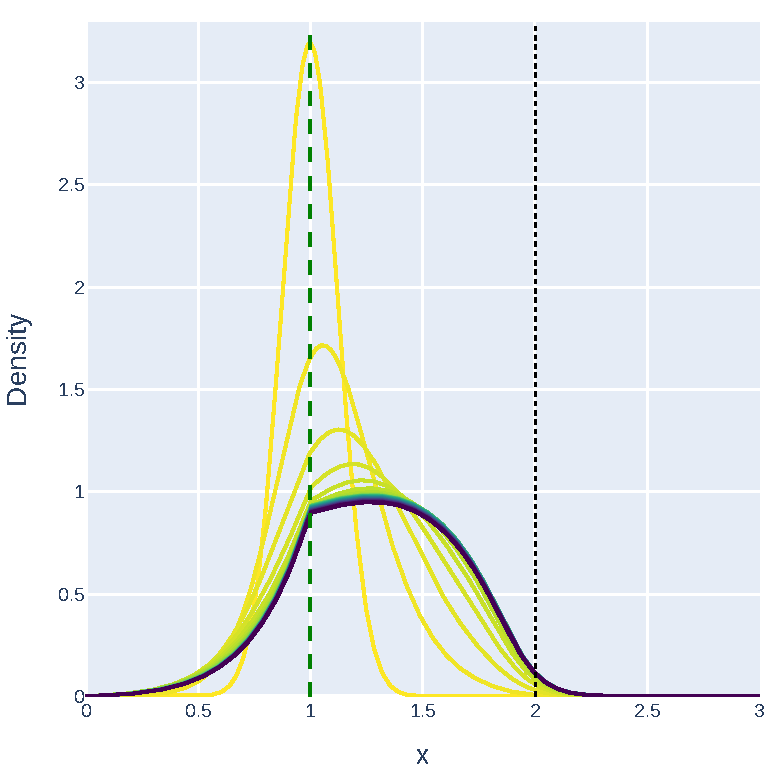
\includegraphics[height=0.25\textwidth]{figures/density_evolution_pois_jump_max_sigma.pdf}}
    \caption{Evolution of the probability density over varying types of stochastic hybrid system on $(-\infty, 2]$}
\end{figure}

\subsection{Geometric Integration for Stochastic Mechanical Systems (Lee)}\label{sec:geo_int}

A significant subclass of stochastic hybrid systems arises from Lagrangian or Hamiltonian mechanical systems with impacts, such as colliding rigid bodies, robotic manipulators with intermittent contact, or locomotion systems undergoing repeated foot-ground interactions. 
These systems exhibit smooth mechanical evolution punctuated by discrete transitions due to impacts, while also being subject to stochastic perturbations from environmental noise or actuation uncertainty. 
The interplay between randomness and nonsmooth transitions introduces analytical and numerical challenges, particularly in preserving the structure and long-term stability of simulations.

For deterministic mechanical systems, variational integrators derived from discretized variational principles are well known for preserving geometric structures such as symplecticity and momentum maps, and for exhibiting good long-term energy behavior. 
Extending these ideas to stochastic mechanical systems has led to the development of stochastic variational integrators, which inherit similar structure-preserving properties in the presence of noise. 
However, when impacts are introduced, standard methods often fail to capture the correct energy and momentum behavior across discrete transitions. 
This motivates the development of stochastic variational integrators that are compatible with impact dynamics, ensuring consistency with the underlying hybrid mechanical structure.

\paragraph{Accomplishments}

This work presents the formulation of stochastic variational impact integrators for hybrid mechanical systems with additive noise~\cite{CLeePIWLHMNC24}. 
Two formulations are considered: one based on the Euler-Lagrange equations derived from a stochastic action principle, and another via the Hamilton-Pontryagin principle on the Pontryagin bundle. 
In both cases, randomness is incorporated through a stochastic potential, while impacts are treated as discontinuities in the trajectory. 
Discretizing these variational formulations yields structure-preserving numerical schemes that respect the hybrid nature of the dynamics and maintain consistent energy behavior over time. 
Numerical simulations demonstrate the effectiveness of these integrators in capturing the long-term statistical and energetic behavior of stochastic mechanical systems with impacts.

\paragraph{Future Directions}

Future work will extend these integrators to mechanical systems on Lie groups, such as rigid bodies and multibody systems with symmetry, as well as systems with holonomic constraints and multiplicative noise. 
Another important direction involves developing adaptive integrators that respond to variability in both noise and impact timing, and conducting rigorous error and convergence analysis. 
Finally, these integrators will be integrated into broader pipelines for stochastic control, reinforcement learning, and model predictive control in uncertain mechanical environments.


\subsection{Geometric Modeling of Deterministic State Uncertainty (Guralnik, Lee)}\label{sec:deterministic_uncertainty}

In many practical applications, modeling uncertainties with a probability density function requires detailed statistical knowledge of the underlying disturbances, which may be unavailable or unreliable.
This is particularly true in systems where data is sparse, measurement noise is non-Gaussian, or rare but critical events dominate the system behavior.
In such cases, a deterministic bound provides a more robust and conservative means of characterizing uncertainty.
By specifying that disturbances lie within a known set—such as a norm-bound or interval constraint—one can design controllers, estimators, and safety guarantees that hold uniformly for all admissible uncertainties, rather than in expectation or with high probability.
This approach is especially valuable in safety-critical systems, such as aerospace or autonomous robotics, where worst-case guarantees are essential.
Moreover, bounded uncertainty models align naturally with set-based and reachability analysis techniques, enabling rigorous verification and robust control design without relying on precise probabilistic assumptions.

\paragraph{Accomplishments \& Directions}

We focus specifically on intermittent state feedback control and estimation, where measurements are available only within a prescribed region, say $D$, but the desired path may lie outside of $D$.
In such cases, control must be computed based on an estimated state whose associated uncertainty bound grows when operating outside $D$.
This creates an inherent conflict: while the control objective drives the system along a desired trajectory outside D, the estimation objective incentivizes visiting the interior of D to reduce uncertainty.
Crossing the boundary of $D$ leads to discontinuities in the estimated state, the uncertainty bound, and the resulting control input—naturally forming a hybrid dynamical system.

Specifically, in the absence of continuous feedback, it becomes necessary to generate dynamic state estimates, which give rise to a region of uncertainty: a time-varying (typically expanding) set that represents an upper bound on all states reachable from a set of initial conditions under admissible control.
Planning and control strategies built on such estimates are inherently conservative, reflecting the minimal observability of the system in this setting.
Nonetheless, they are essential in risk-averse applications where probabilistic guarantees are insufficient due to the high cost of failure.

In practice, intermittent measurements offer discrete opportunities to “chip away” at the region of uncertainty, resulting in improved—though more geometrically complex—state estimates.
These estimates evolve under hybrid, shape-dependent dynamics, and recent findings indicate that control strategies can be extended to handle uncertainty regions with time-varying geometry.
Current efforts are focused on understanding theoretical performance guarantees in the ideal case, where the continuous evolution of the uncertainty region is fully known, as well as more practical approaches where the region is over-approximated by a cover consisting of $N$ balls.
We are also exploring alternative, more efficient representations, such as polynomial zonotopes.
A central objective is to study the tradeoffs between the complexity of the uncertainty region’s representation (e.g., the number N in a ball cover) and the performance of the resulting hybrid controller.
In particular, we consider how topological transitions—such as the uncertainty region fracturing into disconnected components—can trigger estimation updates aimed at reducing the region to a single connected component.

%\subsection{Hybrid dynamic network for DSGRN (Bloch, Mischaikow, Kalies, Guralnik)}\label{dynamic networks in DSGRN}
%%
%\cite{mouyebe2025coupling} investigated the stability and stabilization of coupled network dynamics using Lyapunov methods to prescribe the consequences of coupling effects.
%%
%An interesting challenge addressed are switched network systems, where the network structure can change over time.
%%
%We will study coupled network dynamics from a homological perspective.
%%
%We plan to extend the theoretical framework in DSGRN (\cite{gameiro2024globaldynamicsordinarydifferential}) to recast the problem of changes in network topology as changes in parameters of a larger network.
%%
%This allows one to characterize the global dynamics of switching networks by constructing combinatorial models that preserve algebraic topological invariants across different network configurations.
%%
%This approach will enable us to systematically analyze how network reconfiguration affects equilibria, periodic orbits, and connecting orbits, while identifying critical parameter regions where qualitative changes in system behavior occur.
%%
%%\dg{ALL, I am happy with this version as is, but I must still ask: would you like me to throw strategy spaces into the mix here? Thanks, --Dan. Tony: I would be okay if you added that. }
%%TL: this section is integrated with 3.1

\subsection{Data-driven Learning for Open Hybrid System (Bloch, Ghaffari)}\label{sec:metriplectic}

A metriplectic system is a deterministic framework that combines conservative and dissipative dynamics within a unified geometric structure, making it well-suited for modeling open systems that exchange energy or entropy with their environment.
It augments Hamiltonian mechanics by introducing a symmetric, positive semi-definite bracket alongside the standard Poisson bracket, governed by an energy function (Hamiltonian) and an entropy function.
This structure ensures energy conservation while enforcing entropy increase, consistent with the second law of thermodynamics.
In contrast, stochastic dynamical systems model openness and uncertainty through random processes—such as Brownian motion or Poisson jumps—capturing environmental interactions as probabilistic disturbances.
Dissipation in stochastic systems is not structurally encoded but emerges from statistical noise, making them more flexible for modeling random fluctuations and external uncertainties.
While both frameworks address open-system behavior, metriplectic systems are ideal for studying structured, thermodynamically consistent dissipation, whereas stochastic systems offer a broader probabilistic view of uncertainty in complex environments.

\paragraph{Accomplishments \& Directions}

In our work \cite{teng2024generalized}, we proposed a generalized metriplectic framework that enables the modeling of nonconservative dissipative effects, such as those arising in rigid bodies immersed in fluid, while still preserving thermodynamic consistency.
This is achieved by introducing the concept of free energy—a combination of Hamiltonian and entropy—thereby relaxing the classical requirement that entropy be a Casimir invariant.
This generalization broadens the class of systems that can be described.
To identify unknown components from data, we developed a bilevel convex optimization method that alternates between learning the dissipative metric and the entropy function, both modeled as polynomials.
The approach is computationally efficient, leveraging linear matrix inequalities (LMIs) and linear programs (LPs), and is demonstrated on both planar and rotational mechanical systems on the special orthogonal group.

This work is closely related to \cite{teng2024generalized}, where a metriplectic extension of the Euler–Poincaré equations was introduced, along with structure-preserving discretizations that conserve energy and reproduce entropy production rates, ensuring thermodynamic consistency in numerical simulations.
Currently, we are extending these results to hybrid metriplectic systems involving discontinuities, with preliminary results developed for linear hybrid systems with switching dynamics.

\section{Scalability and Applications}\label{sec:SA}

The \textit{scalability and applications} thrust focuses on developing computationally efficient and theoretically grounded methods for optimal control, learning, and analysis of complex hybrid systems. 
Central to this effort is the Affine Geometric Heat Flow (AGHF) framework, which enables scalable hybrid trajectory optimization by evolving trajectories through PDE-based flows, with extensions to high-dimensional manipulators and humanoid robots (\Cref{sec:affine_geometric_flow}). 
Hybrid Mean Field Games (MFGs) extend classical MFG theory to decentralized control in hybrid systems, with demonstrated applicability to dynamic crowd evacuation scenarios (\Cref{sec:hybrid_MFG}). 
The Discrete Hybrid Automata Learning (DHAL) framework integrates reinforcement learning with hybrid automaton structure inference, enabling robust locomotion control in multi-legged robots (\Cref{sec:DHAL}). 
Concurrently, a generalized extension of DSGRN is being developed to enable topological analysis and verification of hybrid control systems without precise numerical models (\Cref{sec:DSGRN}). 
Finally, a novel HJB-based formulation is proposed to address optimal control in the presence of Zeno behaviors, offering a path forward in systems where traditional necessary conditions break down (\Cref{sec:Zeno}). 
Together, these contributions advance the state-of-the-art in scalable, data-driven, and structure-preserving methods for hybrid control and learning.

\subsection{Scalable Hybrid Optimal Control with Affine Geometric Heat Flow (Vasudevan)}\label{sec:affine_geometric_flow}

Optimizing hybrid trajectories involving discontinuities and discrete transitions is challenging, particularly due to the computational complexity introduced by switching behaviors, impacts, and mode-dependent dynamics. 
Traditional variational and optimal control methods often become intractable or brittle when applied to high-dimensional hybrid systems. 
This motivates the development of scalable computational frameworks that preserve system structure and accommodate nonsmooth behavior. 
The following work addresses these challenges by leveraging PDE-based formulations and trajectory-centric optimization techniques that scale efficiently and generalize across a wide range of hybrid dynamical systems.

\paragraph{Accomplishments}

Specifically, we have introduced a new PDE-based framework for trajectory optimization called Affine Geometric Heat Flow (AGHF).
The central idea is to evolve a trajectory toward optimality by treating it as the solution to a parabolic partial differential equation on a 2D domain, where the pseudo-time variable drives the deformation of an initial path into one that satisfies both the system dynamics and boundary conditions.
Under mild conditions on the dynamics, one can prove that this approach will converge to a feasible trajectory if one exists.
This method offers a scalable alternative to traditional Hamilton-Jacobi or Pontryagin-based techniques, which can be computationally intractable for high-dimensional systems.
Notably, AGHF does not require solving over the full state space but instead operates directly on the trajectory as a whole.

Building on this theoretical foundation, the PHLAME (Phasing Through the Flames: Rapid Motion Planning) framework \cite{adu2025phasing} introduced a pseudospectral implementation using Chebyshev collocation methods and spatial algebra to accelerate the solution process, achieving order-of-magnitude improvements in runtime.
A related formalism, BLAZE \cite{adu2025bring}, generalizes the objective function to allow arbitrary cost functionals and incorporates a two-phase optimization procedure.
This two-phase method first ensures feasibility—even from constraint-violating initial guesses—and then refines the trajectory for optimality.
These methods have been demonstrated on a variety of systems, including manipulators with over 20 degrees of freedom and humanoid robots, achieving constraint-satisfying, dynamically feasible trajectories in as little as 2–5 seconds.
Importantly, input and state constraints—including actuator limits and collision avoidance—are natively handled within the optimization.
We have also extended these approaches to hybrid systems with impacts, under the assumption that the number and sequence of contacts is specified a priori.

\paragraph{Future Directions}

Our ongoing research seeks to extend the AGHF framework to hybrid systems with impacts and discrete transitions where the contact sequence is not specified a priori.
One promising direction is to couple the AGHF evolution with a complementarity-style formulation, incorporating reset maps directly into the PDE or into the phase structure used in BLAZE.
Additionally, we are investigating whether the two-phase approach developed in BLAZE—first projecting to the feasible set, then optimizing—can be extended to systems exhibiting Zeno behavior or those with an unknown number and timing of impacts.
This would enable the treatment of trajectories involving a variable number of discrete events, such as multi-bounce systems or hybrid transitions under uncertainty.
Our goal is to create a numerically robust framework for hybrid optimal control that leverages the computational advantages of AGHF while integrating the structural insights of hybrid systems theory.

\begin{figure}[b]
\begin{minipage}{0.6\textwidth}
    \centering
    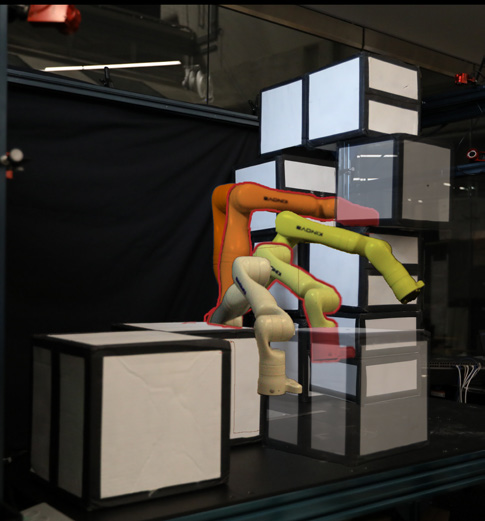
\includegraphics[height=3.1cm]{figures/aghf-000.png}
    %\includegraphics[height=3.1cm]{figures/aghf-001.png}
    
\includegraphics[height=3.1cm]{figures/aghf-004.png}
    \caption{Optimal trajectories in a higher-dimensional space constructed by affine geometric heal flow~\cite{adu2025bring,adu2025phasing}}
\end{minipage}
\hfill
\begin{minipage}{0.35\textwidth}
    \centering
    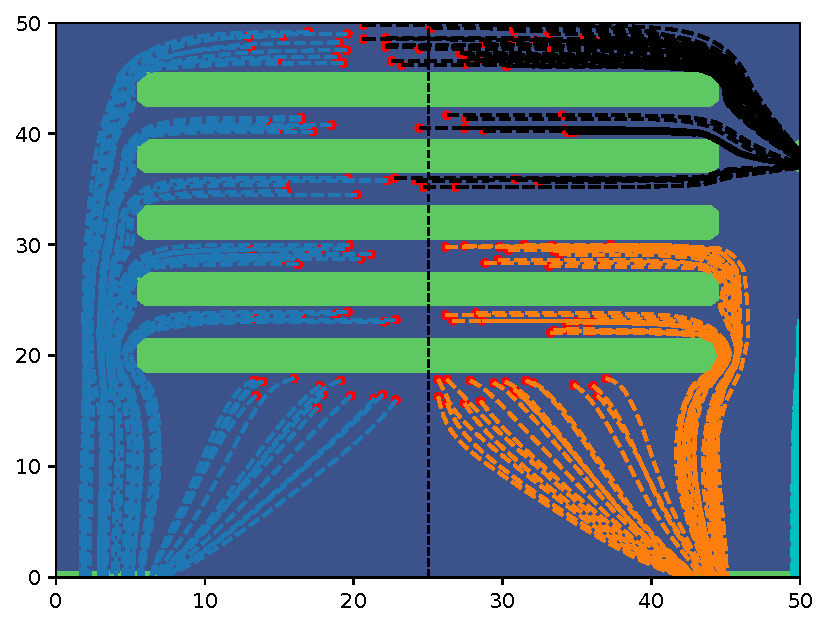
\includegraphics[height=3.1cm]{figures/MFG/sample_traj_HybMFG.pdf}
    \caption{Hybrid mean field game for crowd evacuation utilizing hybrid structures}
\end{minipage}
\end{figure}

\subsection{Hybrid Mean Field Game (Lee)}\label{sec:hybrid_MFG}

Mean field games (MFGs) for hybrid systems extend classical MFG theory to settings where each agent evolves according to hybrid dynamics—that is, systems that combine continuous evolution (e.g., differential equations) with discrete events (e.g., mode switching, impacts, or jumps).
In this framework, each agent optimizes its own cost while responding to the aggregate behavior of a large population, represented by a mean field.

Incorporating hybrid dynamics into MFGs introduces significant complexity.
Mode-dependent dynamics, guards, and reset maps must be accounted for in both the agent’s optimal control problem and the evolution of the population density.
These features make hybrid MFGs particularly suitable for modeling large-scale, decentralized systems in which agents interact under mixed discrete-continuous behaviors—examples include traffic networks, multi-agent robotic systems, and cyber-physical infrastructures.
The hybrid MFG framework enables scalable analysis and control of such systems, providing insights into their collective behavior and supporting the design of distributed strategies that are optimal in the limit of large populations.

\paragraph{Accomplishments \& Directions}

In \cite{CLeePISNCS25}, we presented the governing equations for hybrid mean field games and control, consisting of a set of coupled partial differential equations: a hybrid Hamilton-Jacobi-Bellman (HJB) equation describing the optimal control of a representative agent, and a hybrid Fokker-Planck equation describing the evolution of the population’s density across both continuous and discrete states.
These equations build on earlier work that formulates the transfer operators for stochastic hybrid systems, as discussed in \Cref{sec:SHS}.

We applied this framework to a crowd evacuation scenario, where each agent (individual) aims to minimize evacuation time while navigating around obstacles toward exits, and avoiding crowded regions that inhibit rapid movement.
The system exhibits hybrid dynamics due to two key features.
First, abrupt changes in exit configurations—such as exits opening, closing, or relocating due to environmental conditions (e.g., fire spread, blockages, or emergency protocols)—induce discrete mode switches that affect control options and cost landscapes for all agents.
Second, a hypothetical teleportation mechanism allows an individual to be reset to another location, such as closer to an exit or into a less congested area.
This is modeled as a jump triggered by a guard and a corresponding reset map in the hybrid system.

Numerical simulations illustrate the optimal behaviors of individuals that fully exploit the hybrid structure.
For example, one group gathers near an area where a new exit is expected to open, while another group takes a shorter path via the teleportation mechanism.
These results demonstrate scalable, decentralized decision-making in highly dynamic and constrained evacuation scenarios, explicitly leveraging the unique features of hybrid systems.
Ongoing work focuses on developing scalable computational techniques applicable to complex hybrid systems on higher-dimensional manifolds.

\subsection{DHAL: Discrete Hybrid Automata Learning (Ghaffari, Mischaikow, Kalies, Clark)}\label{sec:DHAL}

The learning and control of multi-legged robots with contact pose significant challenges due to the hybrid nature of locomotion, which combines continuous body dynamics with discrete events such as foot touchdown and lift-off.
These contact transitions induce frequent mode switches that are inherently non-smooth and analytically difficult to model.
The underlying dynamics are high-dimensional, underactuated, and often involve complex frictional interactions, limiting the effectiveness of standard gradient-based optimization techniques.
Moreover, contact sensing is typically noisy or delayed, complicating both state estimation and feedback control.
Coordinating multiple limbs under these conditions requires robust, adaptive control policies that generalize across varying terrains and gait patterns.
Addressing these challenges necessitates a principled integration of hybrid dynamical systems theory with data-driven learning approaches to achieve reliable and efficient locomotion.

\paragraph{Accomplishments}

To this end, we developed the Discrete-time Hybrid Automata Learning (DHAL) framework~\cite{liu2025discrete}, with robotic skateboarding as a motivating application.
DHAL is a reinforcement learning framework that jointly learns the hybrid automaton structure (i.e., mode transitions), the continuous dynamics within each mode, and the corresponding hybrid control policy.
Notably, DHAL does not require pre-labeled mode annotations.
Instead, it employs unsupervised learning to identify and select discrete modes.
A probabilistic policy, modeled using a beta distribution, is trained in conjunction with a multi-head critic network, enabling end-to-end learning from raw interaction data.
The discrete-time formulation naturally captures the hybrid structure of the dynamics and facilitates efficient policy optimization.

This framework integrates hybrid automata models with reinforcement learning, allowing robots to adapt to dynamic and contact-rich environments, such as snowy slopes, without relying on predefined trajectories or event labels.
By enabling interpretable, mode-aware interaction with the environment, DHAL supports explainable decision-making in complex scenarios.
We validated the approach on a quadrupedal robot executing advanced skateboarding maneuvers.
Through a multi-critic training strategy—rewarding gliding, pushing, and successful sim-to-real transfer—the robot demonstrated the ability to navigate diverse terrains and withstand disturbances, while maintaining robust performance.
This work advances the scalability and verification of open hybrid systems by explicitly identifying task-level motion modes and leveraging them for control.

\paragraph{Future Directions}

Looking ahead, we aim to integrate DHAL with the homological analysis methods described in \Cref{sec:learning_Mischaikow}.
In particular, DHAL’s data-driven decomposition of trajectories into discrete modes and mode-specific dynamics can be directly leveraged to build mode-aware cellular decompositions of hybrid phase space, enabling computational topology techniques such as Conley index theory.
This integration would allow estimation of invariant sets, attractors, and their connectivity, thus uncovering global structures in hybrid dynamics.
Such a unified approach offers both local (mode-level) and global (system-wide) insight, facilitating verification, control synthesis, and refinement of hybrid models from data, with topological feedback guiding learning and adaptation.

\begin{figure}
    \centering
    
\includegraphics[height=3cm]{figures/dhal-000.png}
    \hfill
    
\includegraphics[height=3cm]{figures/dhal-003.png}
    \hfill
    
\includegraphics[height=3cm]{figures/dhal-008.png}
    \caption{Discrete Hybrid Automata Learning (DHAL) framework illustrated by robotic skateboarding~\cite{liu2025discrete}}
\end{figure}

\subsection{Generalized DSGRN for Hybrid Control (Guralnik, Mischaikow, Kalies)}\label{sec:DSGRN}

The power of DSGRN is that it starts with a network model that indicates which variables are influencing which other variables.
From the network a cubical complex and a parameter space (represented by a graph) is constructed.
This purely combinatorial/homological structure is used to perform computations to characterize the dynamics over different parameter regions.
The combinatorial model for dynamics is constructed to model a flow generated by an ODE.
After the computations are performed, this abstract structure is given a geometric realization in such a way that one can draw rigorous conclusions about the continuous process.

\paragraph{Accomplishments \& Directions}

Overall, the algebraic topological study of our project is to build a similar framework for hybrid systems.
We have a mathematical structure to work with: the graph in the product complex of the combinatorial model.
For the continuous part of the dynamics we expect it will take a similar form as DSGRN and 
the model of behavior at guards should follow that of combinatorial models for dynamics generated by continuous maps.
One challenge is that our algorithms are not designed work with this type of hybrid system and preliminary work suggests that the homological interpretation of dynamics can be significantly different from that of traditional dynamical systems.

Another challenge is that discretization limits the possibilities for control, as input values are selected as functions of just the discrete state.
In the case of DSGRN, regarding some of the system parameters as control inputs gives rise to a discrete transition system embedded in the product of the cubical complex with the parameter space.
Continuity of control may then be approximated using the graph structure of parameter space, but this kind of control---whether implemented in reality using piecewise-constant inputs or otherwise---is inherently hybrid.


Consequently, two goals arise: obtaining a valid extension of DSGRN's way of discretizing parametrized dynamics over general open hybrid systems, and obtaining means for analysis of closed-loop behaviors in such systems.
In other words, we are developing tools to analyze closed-loop behavior and controllability using topological and graph-based methods, and enabling scalable and verifiable computation of hybrid system behaviors without requiring precise numerical models
In particular, one direction of current inquiry is the understanding of controllability properties of DSGRN instances as a function of the underlying interaction/interconnection graph, using strategy spaces, and in line with the goals of \ref{sec:dynamic networks in DSGRN}.

\subsection{Hybrid Optimal Control with Zeno Behaviors (Vasudevan, Clark)}\label{sec:Zeno}

Zeno behavior—where a hybrid system exhibits an infinite number of discrete transitions in finite time—poses fundamental challenges to both the analysis and optimal control of hybrid systems. 
Traditional optimal control frameworks often assume a finite number of mode switches or regularity in switching times, assumptions that break down in the presence of Zeno phenomena. 
Yet, Zeno behavior arises naturally in many real-world systems, such as mechanical systems with impacts, relay circuits, and certain robotic locomotion strategies, where chattering or rapid switching may be energetically favorable or necessary to achieve fine control. 
Ignoring such behaviors can lead to overly conservative solutions or complete failure of standard algorithms. 
Therefore, developing a rigorous and computationally tractable framework for incorporating Zeno dynamics into optimal control is crucial for advancing the reliability and performance of hybrid systems in safety-critical applications. 

\paragraph{Accomplishments}

Specifically, classical tools for hybrid optimal control, such as the hybrid maximum principle and dynamic programming formulations via the Hamilton-Jacobi-Bellman (HJB) equation, typically assume that discrete events are uniformly separated. 
In particular, the hybrid maximum principle fails in the presence of Zeno trajectories, as shown in prior work~\cite{clark2023optimality}.
In this research thrust, we explore the applicability of the HJB framework to hybrid systems that exhibit Zeno behavior.
We consider the controlled bouncing ball as a canonical testbed: a system whose trajectories necessarily undergo infinitely many impacts as they converge to a rest configuration. 
By formulating the hybrid HJB equation with appropriate boundary conditions at the guard and its image, we are able to define a value function that remains meaningful even as trajectories approach the Zeno limit. 
Using a semi-Lagrangian upwind numerical scheme, we compute the value function and investigate how optimal controls behave in the Zeno regime. 
Our results indicate that it is possible to approximate value functions for such systems despite the breakdown of traditional necessary conditions, opening a new pathway for optimal control of Zeno systems.

\paragraph{Future Directions}

We are currently validating our numerical algorithm on both simulated and physical systems to confirm its correctness in approximating the hybrid HJB value function near Zeno states. 
One of our goals is to characterize the qualitative structure of the value function near the Zeno point and to identify features such as sensitivity to initial conditions and the emergence of multiple local minima corresponding to different impact patterns.
We are also exploring how this approach generalizes to other hybrid systems, including those with nonholonomic constraints or impacts between multiple bodies.

%TL: the following two topics can be included in the next report. 

%\subsection{Hybrid rigid body optimal control (Ghaffari, Vasudevan, Lee)}\
%We developed certifiable globally optimal trajectory optimization for multi-body systems~\cite{teng2024convex} and a fast Riemannian solver on Lie groups for direct trajectory optimization~\cite{teng2025riemannian}. The two works are complementary, i.e., global and local search. We will work on extending these to a hybrid setting, e.g., mechanical systems with contact.

%\subsection{Invariant filtering for hybrid dynamic network (Lee, Ghaffari)}
%We will study the extension of invariant and equivariant observers to hybrid systems, e.g., under a change of locomotion mode or moving ground. A more general setting would be hybrid systems in non-inertial frames, and we may explore it. We developed a maximum entropy filter~\cite{teng2025max} that can track polynomial systems under arbitrary noise distributions. We plan to extend the framework to stochastic hybrid systems and their connection with Lie theory for equivariant systems. 

\printbibliography

\end{document}

